\chapter{Train Benchmark Implementation}

\section{Original Version}

\subsection{Framework}

\begin{figure}[!Htb]
	\centering
	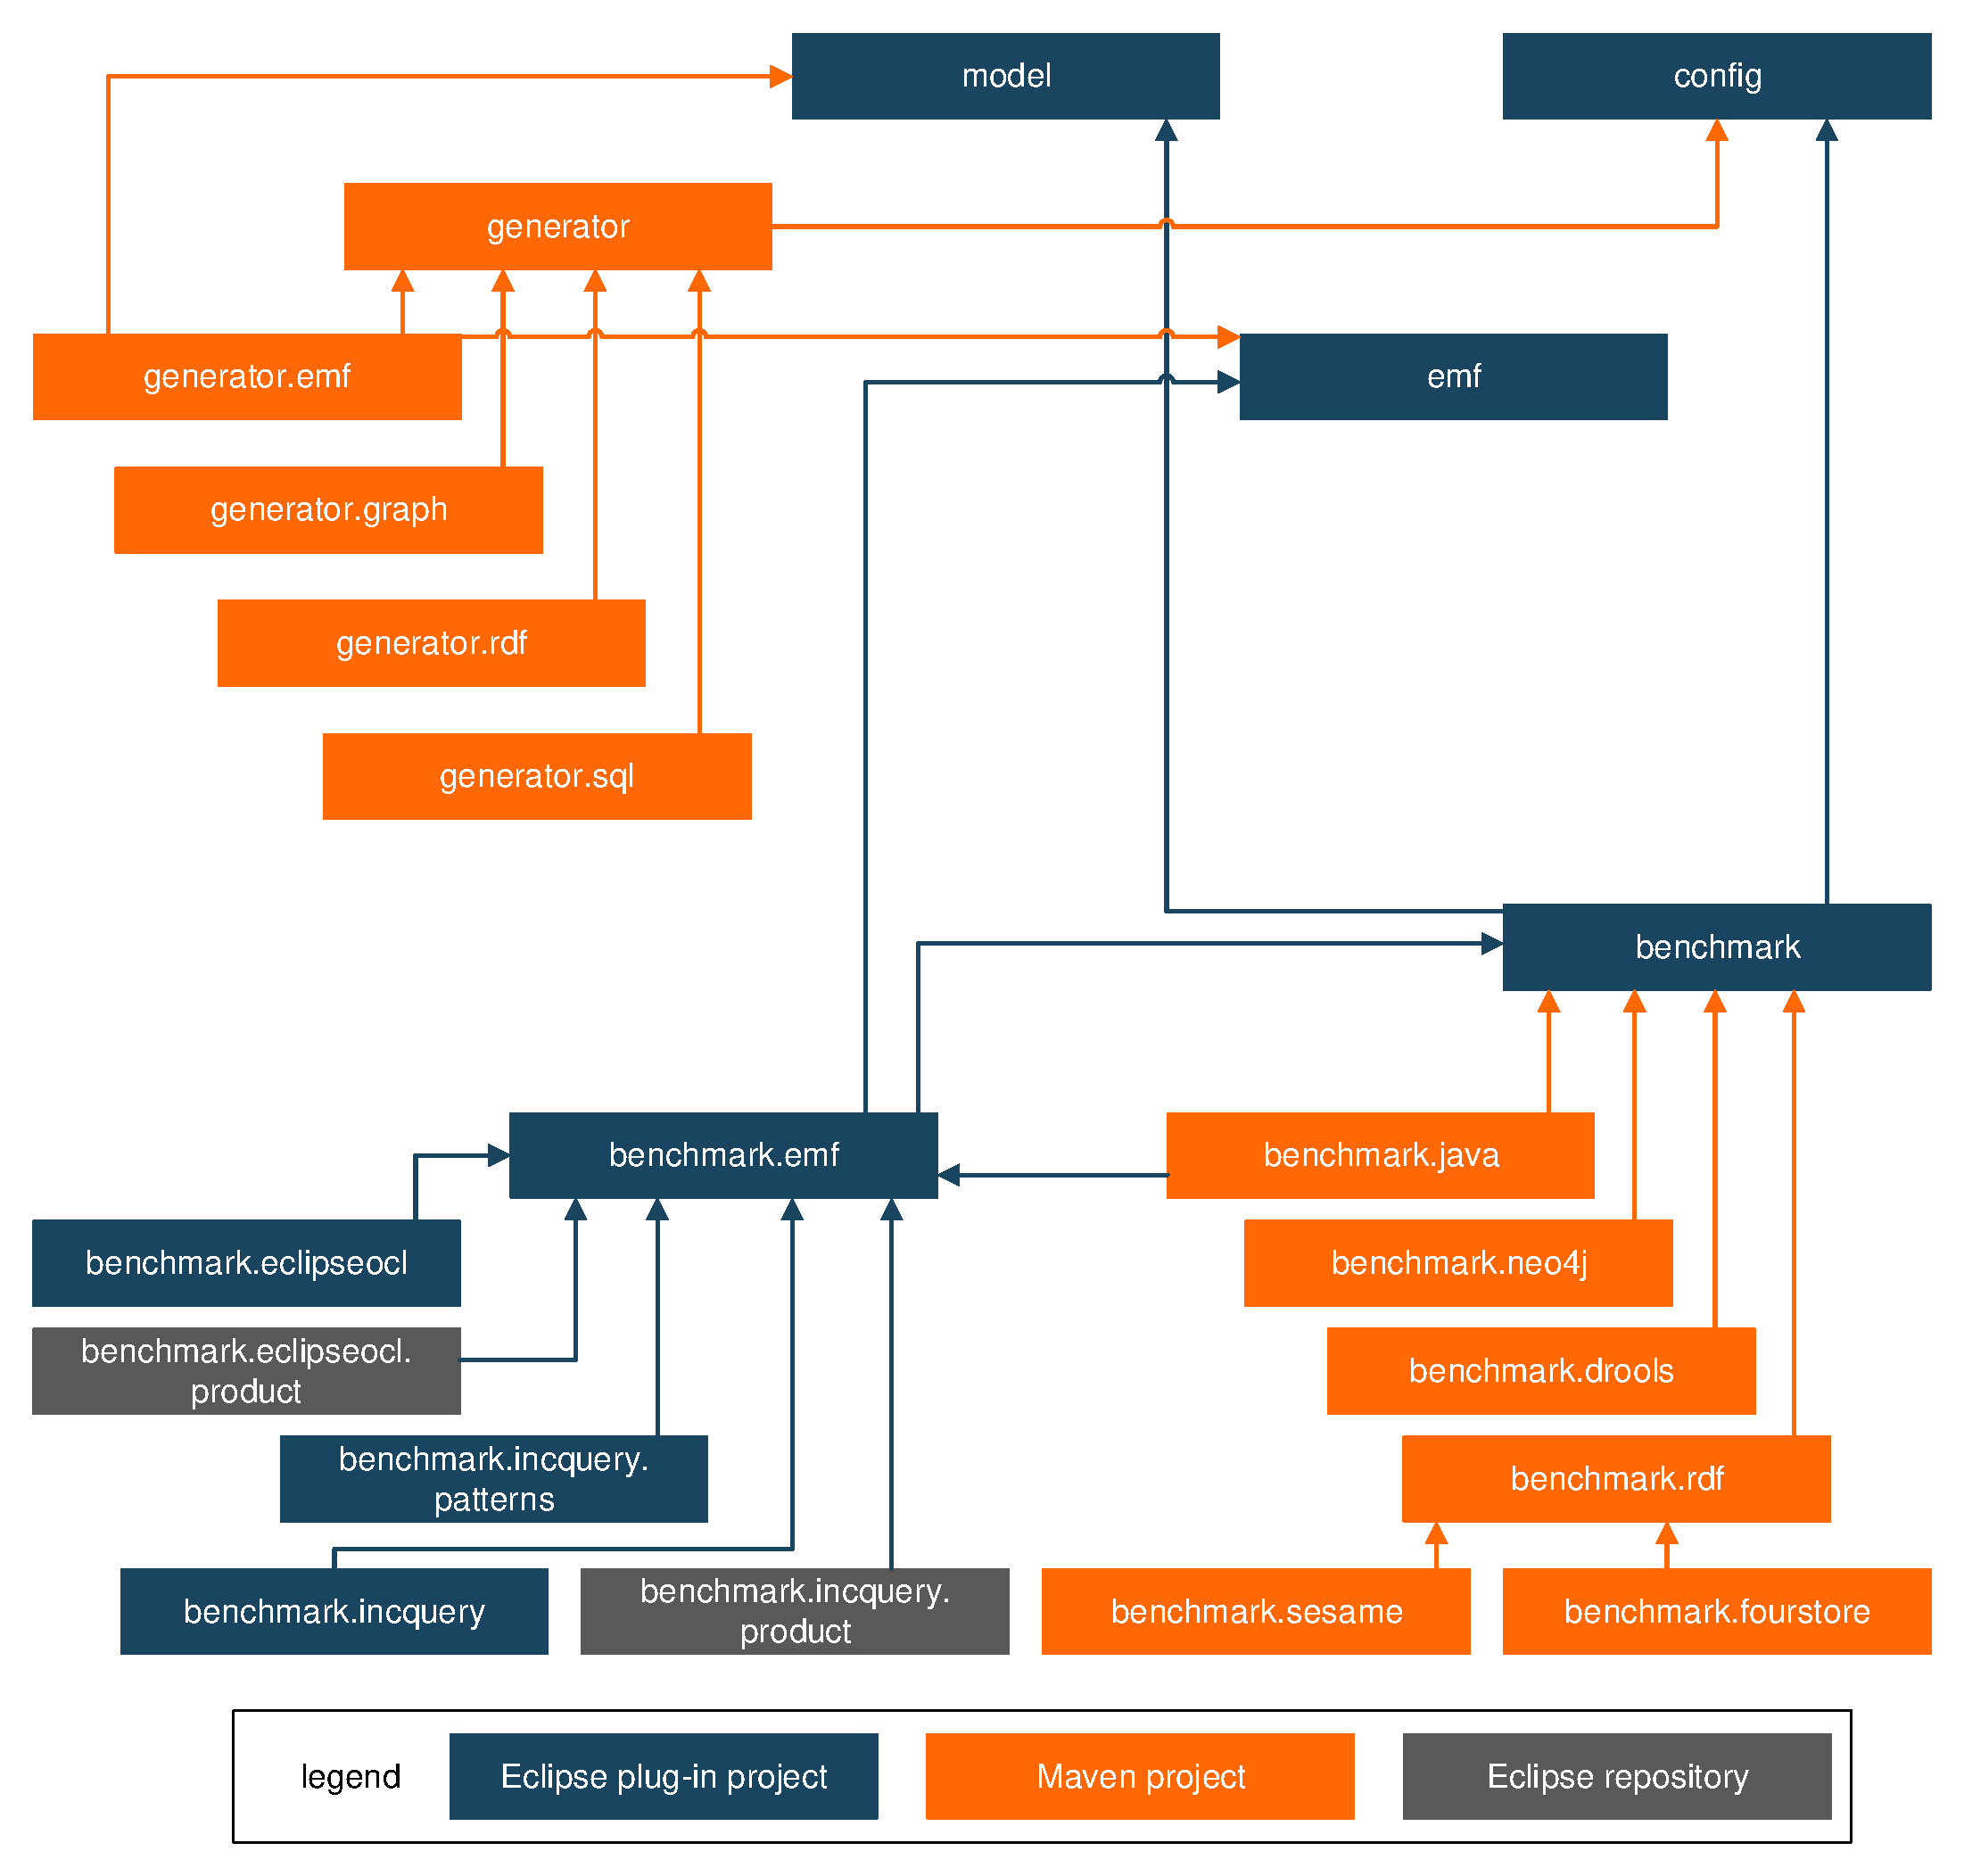
\includegraphics[width=\textwidth]{figures/trainbenchmark-modules}
	\caption{The Maven modules defined in the Train Benchmark. Note that artifact ids of the modules are abbreviated and their full id starts with \texttt{hu.bme.mit.trainbenchmark}.}
	\label{fig:trainbenchmark-modules}
\end{figure}

\subsection{Architecture}

For the integration of the Train Benchmark projects and their third party dependencies, we use Apache Maven~\cite{Maven}. The dependencies are shown in \figref{fig:trainbenchmark-modules}.

In this section, we briefly describe each module's tasks and responsibilities.

\subsubsection{Parent module}

The \texttt{hu.bme.mit.trainbenchmark} module is the parent module which contains the modules used in the Train Benchmark. Building this Maven module builds all child modules as well.

\subsubsection{Central modules}

The \texttt{hu.bme.mit.trainbenchmark.model} module contains the reference metamodel represented in EMF.

The \texttt{hu.bme.mit.trainbenchmark.config} module contains classes and constants used by the \emph{generator} and the \emph{benchmark} projects.



\subsubsection{Representation-specific modules}

The \texttt{hu.bme.mit.trainbenchmark.emf} and \texttt{hu.bme.mit.trainbenchmark.rdf} modules contain classes and constants used by the particular representations.



\subsubsection{Generator modules}

The \texttt{hu.bme.mit.trainbenchmark.generator.*} modules are responsible for generating the instance models for the benchmarks.

\begin{itemize}
  \item \texttt{emf}: generates an EMF instance model.
  \item \texttt{graph}: generates a property graph model in the specified format: GraphML (default), Blueprints GraphSON, Faunus GraphSON.
  \item \texttt{rdf}: generates an RDF instance model.
  \item \texttt{sql}: generates an SQL script which creates and loads the appropriate database tables.
\end{itemize}



\subsubsection{Benchmark modules}

The \texttt{hu.bme.mit.trainbenchmark.benchmark.*} modules are responsible for benchmarking. For the list of current implementations, see \ref{tools}.


\subsection{Services}

\subsection{API}

\subsection{time meas}

To obtain faithful execution times, we implemented a benchmarking framework,
which accounted for the time measurements with nanosecond precision (however, the accuracy may be lower than that),
 and the clear separation of phases enforced by the defined
interfaces. These model loading and querying functions were implemented using
functionally equivalent calls of a given tool. See Table~\ref{table:tools} for
the model management format and query language of the benchmarked tools. The
benchmarks were realized as Java applications.

\subsection{memory meas}
Before acquiring memory usage (free heap space) from the JVM, GC calls were triggered five times to sweep unfreed objects from the RAM.

\todo{+init +destroy, getmemusage, getbmr, \ldots}
Before every test
there is an unmeasured initialization phase. Environment initialization
instructions are executed, like clearing the OS file cache, triggering the
execution of the garbage collector, and starting server processes outside the
JVM if necessary (for example the Virtuoso server). At the end of each benchmark
in a separate unmeasured phase memory usage is measured (after calling the GC),
and finally network connections are closed, data structures are disposed, and
separate server processes are stopped.


\section{Discussion of fairness considerations}
Many different tools are measured in the benchmark which have various strenghts
and weaknesses. Model and query description languages have different expressive
power, however the benchmarking data model and queries are expressible in all
languages: executing them they return the correct number of invalid elements,
and semantically they are mapped as closely as languages enable, without using
cumbersome, unnatural expressions in a language.

EMF provides a class diagram like metamodel description language. Objects are
classified into classes, and connections between them are described by relations
(or attributes, when the target object's type is not a class, but a primitive
type, e.g. EInt). Enumerations, generalizations between classes, inverse
relations and simple cardinality restrictions are supported. Flat containment
hierarcy is used: a special class instance is created as the root object which can
hold all individuals. On the instance level EMF objects and instance relations
are created between them as described in \secref{sec:instanceGeneration}.

In ontologies, the OWL2 language supports all constructs that can be expressed in
EMF, thus the EMF metamodel is mapped to OWL2 TBox. The mapping is done by hand as
described in Sec. 16 of \cite{OMG2009ODM}. Ontology instance model elements are
generated equivalently to the EMF objects. Since an OWL2 file can be serialized
into RDF/XML, the same file is used as input for RDF databases and OWL
reasoners.

Neo4j defines a vertex-attributed, edge-labeled graph structure for describing
models. Here instance objects can be mapped to graph nodes, and instance
relations to graph edges. Metamodel information can be introduced into the graph
as labels. Key-value labels of nodes describe their types, instance names or
value of attributes (like the length of a Segment). The type of an edge can be
given as a label. Initially the generated model is loaded from a GraphML file,
which is also in XML syntax, as RDF/XML or XMI for EMF.

For the SQL test a custom relational schema is created as metamodel. Instance
model elements are stored in records, while primitive type attributes as
attributes, and relations as joins between tables. The input is also a textual
file, but it is not in XML format, it consists of SQL insert commands.

Queries are formulated similarly for the benchmarked tools. Variables are used
to bind them to objects. Types of variables and relation types between two
variables are constrained. For integer checks special check/filter constraints
are used; while the absence of instance model structures are described with
negation in all languages.

\todo{Az alábbi bekezdésből jön implementációs feladat, vagy a threats to validity-ben kell róla valamit írni?}

Of course unique feature of tools or lack of language expressiveness is not
highlighted in the benchmark, in order to be able to compare them. For example,
object type constraints are prescribed in the query, where the language allowed.
However in Java and OCL they are omitted, since it would be strange to read
unnecessary \emph{instanceof} and \emph{oclIsKindOf} expressions. On the other
hand, Drools requires these constraints, as variables are bound based on the
class it belongs to, and relation constraints can be expressed with this given
information. While EMF and OWL supports cardinality constraints and inverse
relations, RDF/RDFS does not support it. The former is not tested in the
benchmark, and the latter can be worked around by switching the subject and
object variables in a SPARQL query.
The handling of types and subsumption hierarchies were crucial for the
benchmark, and fortunatelly it is supported by most languages, although
reasoning capabilities must be turned on for ontology tools to work with this
implicit information. Other extra strengths special for a given tool were not
used, like complex cardinality constraints or transitive closure axioms in
ontology, transitive closure of the IQPL query language, or high availability
modes of Neo4j.

% OCL: org.eclipse.ocl.ecore.source_3.2.0.v20120522-1637.jar/org/eclipse/ocl/opposites/


\begin{figure*}[Hht]
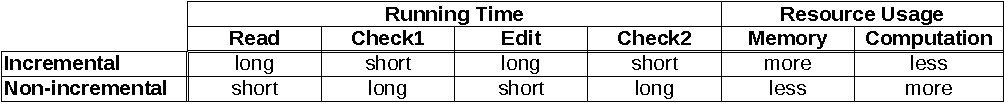
\includegraphics[width=2\columnwidth]{figures/incNonInc.pdf}
\caption{Incremental and non-incremental approaches}
\label{table:incNonInc}
\end{figure*}

Incremental and non-incremental engines use different computational approach,
which results in different characteristics as described by
\figref{table:incNonInc}. A clearly non-incremental tool does no extra work
during the load or modification of the model, but parses it into its memory, and
modifies the structure. In contrast an incremental tool usually builds some
auxiliary data structure (e.g. caches or indexes) on load, and maintains this
during modification (besides performing the modification) resulting in longer
running time. On the other hand incremental tools can return results quickly,
because they only read it from cache, or perform queries using the auxiliary
information (for fast access provided by indexes, utilize scope reduction or
rule reduction techniques). However, non-incremental tools must traverse the
whole model to search for invalid elements resulting in longer query answering
time. In conclusion, incremental tools usually needs less computation time when
the task is not batch dominated (i.e. there are no large transactions with rare
queries), while non-incremental tools need less memory (because there are no
auxiliary helper structures). This is why read+check1 and edit+check2 aggregated
values are used to compare all kind of tools.

Another differentiating factor can be query optimizaton. Formulating the same
constraint using different query primitives or different query ordering can
effect query performance highly. In the field of relational databases it has a
great literature used in tools (like MySQL, or the RDB backed Virtuoso), while
for graph query languages there are less research done in this field. 
\todo{cite needed} In the benchmark\ldots \todo{mit is kezdtünk vele\ldots}

\section{Questions to answer / Related work\ldots / Motivation (todo disassemble)}

\subsection{Why not existing benchmarks?}

There are already available benchmark definitions, however we created a new one
for measuring different tool capabilities. One of the most well known RDF
benchmark is the Berlin SPARQL Benchmark (BSBM) \cite{BerlinBenchmark}, which
models an e-commerce use-case. BSBM concentrates on throughput performance (in a
steady state) of parameterized queries, while our benchmark measures batch and
incremental query evaluation performance of fixed constraint checking queries.
The SP$^2$Bench \cite{SP2Bench} works on an unstructured dataset (DBLP) suited
for RDF data representation with the goal of measuring query evaluation
performance of SPARQL engines, concentrating on testing every feature of the
SPARQL language. In opposite, our benchmark queries a structured dataset, which
queries can be implemented in multiple query and data description languages.
Moreover, our benchmark scenarios address continous evolution of the dataset,
which is a future work in SP$^2$Bench, and also not addressed in \cite{SIB} and
\cite{DBpediaSparql}.

Other ontology benchmarks are the Lehigh University Benchmark (LUBM)
\cite{LUBMBenchmark}, and its improved version, the UOBM Ontology Benchmark
\cite{UOBM}. These are tailored for measuring reasoning capabilities of ontology
reasoners, while our goal is to compare query answering performaces.

Model transformation tools are compared annually in the Transformation Tool
Contest \cite{TTC} by solving model synchronisation, model execution and
simulation, verification use-cases from different application domains. The aim
is to compare expressiveness, usability and performance of different
tools in the field. \todo{kiegészíteni, +hivatkozás}

From the EMF domain we have not found general application benchmarks, or
comparison of EMF query technologies (like Eclipse OCL or EMF Query). However
there are performance measurements \cite{EMF-performance} about core EMF
functions, and different EMF configurations. We tried some relevant
configuration from these tips, but they were not effective, so we stuck at the
default EMF implementation.

We have not used relational database benchmarks, because the main scope of this
article are graph-based databases, and MySQL was included only for a rough
comparison. RDB benchmarks usually use relational schemas (and not graph-based
metamodels), and measure throughput with concurrent modifications like as
defined in the TPC-C \cite{tpc-c} benchmark.

Egyed published papers about verifying and fixing inconsistencies in UML models
\cite{Egyed-fixingInconsistencies, Egyed-instantConsistency} with performance
and memory consumption measurements \cite{Egyed-incConsistency} of the
UMLAnalyzer tool. They measured 19 rules and 30 independent UML models, scaling
up to $100 000$ elements. The tool evaluates OCL expressions in sub-millisecond
time using an impact analyzer approach.

Praxis \cite{falleri-praxis} use rule-reduction technique to provide incremental
instance model validation. It represents the model and edits using an operation
based approach. Technically Java, UML or Movida metamodels can be used, and
conforming instances as well as edit operations are translated to Prolog facts.
Constraints are represented as prolog rules, which are evaluated when they are
triggered based on the user written impact list. The paper reports evaluation
performance in the 0.1 second range (without measuring the conversion time), and
very low (below megabyte during evaluation, and tens of megabytes during
modification at maximum) memory usage.

To summarize, our benchmark concentrates to the model validation use-case, where
constraints (formulated as queries) are fixed, and instance models are evolving.
The benchmark measures the batch phase and incremental phases separately, and
evaluates them for multiple modeling domains (EMF, RDF, OWL, GDB, RDB).

% Social Network Intelligence Benchmark (SIB):
%   Olyan kérdéseket gyűjtöttek, ahol SPARQL jó. _Csak query_, throughput. (Ügyes SPARQL konstrukciók.)
% DBpedia SPARQL Benchmark:
%   Csak query, throughput. De real world.

\subsection{Why this specific domain?}
This domain is selected because it is small (contains only nine concepts), easy
to understand, and no deep domain knowledge is required. All queries can be
expressed over the described metamodel, and the railway terms suggest the field
of critical (or critical embedded) systems, where instance model validation is
used during the software development process.

\subsection{Why these instance models?}
Instance models are generated systematically from pre-defined blocks. This
reflects how large models of common design applications are built: domain
engineers connect modules with minimal variations, chosen from predefined
library elements. Large number of instance model elements can also be
auto-generated by a program, which connects building blocks created from
templates.

\subsection{Are these queries representative?}


% MORE threats : )
We tried to mitigate \emph{internal validity} threats by reducing the number of
uncontrolled variables during measurements: a physical machine was used with all
unnecessary software components turned off and every execution was isolated into
a freshly initialized JVM.

The queries are semantically equivalent in the different query languages and the
result sets are the same for every model. Additionally, to ensure comparable
results the created high-quality query implementations were reviewed: the OCL
implementation by Ed Willink from the Eclipse OCL project, the usage of Impact
Analyzer by Axel Uhl from the Impact Analyzer developer team. The graph patterns
were written by the developers of \incquery{}.

The metamodel and the query specifications were motivated by an industrial case
study, and the selected queries feature commonly used validation tasks such as
attribute and reference checks or cycle detection. We tried to ensure that the
instance models have a similar structure and distribution to other models by
parameterizing the generation process based on our experience with other
domains. To summarize, we believe that the train domain and the generated
instance models represent other domain-specific languages and available instance
models well.

Our current measurements only loaded and executed a single query in each run.
When loading multiple queries, query interference may change the results
greatly. A more detailed evaluation of this issue is planned for the future.

Considering resource-constrained environments, we believe that limiting
available memory will alter the results the most, as the memory management
overhead will reduce the performance of \incquery{}.

It is important to note that heap usage were measured after executing a garbage
collection, so these measurements do not contain memory usage of temporary
constructs. This means that maximum heap usage might have been larger. Furthermore,
limiting heap space by the maximum usage results in excessive garbage collection
and thus an increased runtime. However, in our experience setting the limit to
two times the measured values, such issues do not occur.

In case of the benchmark queries, we measured a $1.5$ GB heap size in case of a
model with $3.5$M model elements that we believe is manageable in a developer
machine with 4--8 GB of RAM. On the other hand, when handling such large
models the existing user interface itself could become a bottleneck. Thus we
believe, our measurement results hold also in the integrated development
environments.
